\begin{appendices}

\chapter{Description du sujet}
\label{appendix:description}

\begin{figure}[h]
  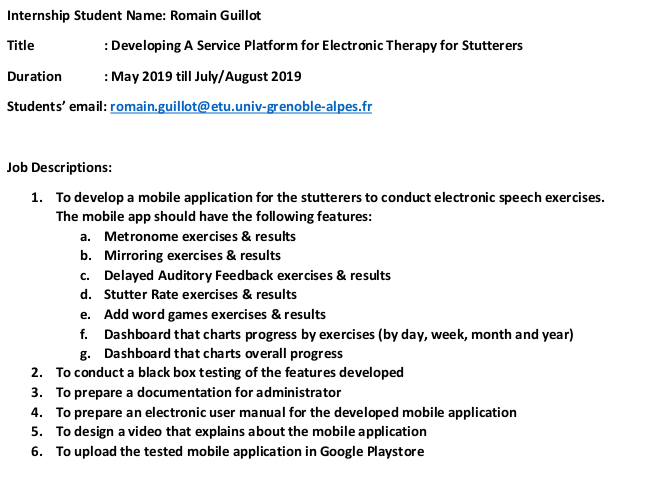
\includegraphics[width=1\linewidth]{content/imgs/description.png}
  \caption*{Description du projet proposé par ma superviseure Dr. Noreen Izza Arshad}
\end{figure}


\begin{landscape}
\chapter{Stutter Manager v3}
\label{appendix:old_app}

\begin{figure}[h]
  \centering
  \begin{subfigure}{.25\textwidth}
    \centering
    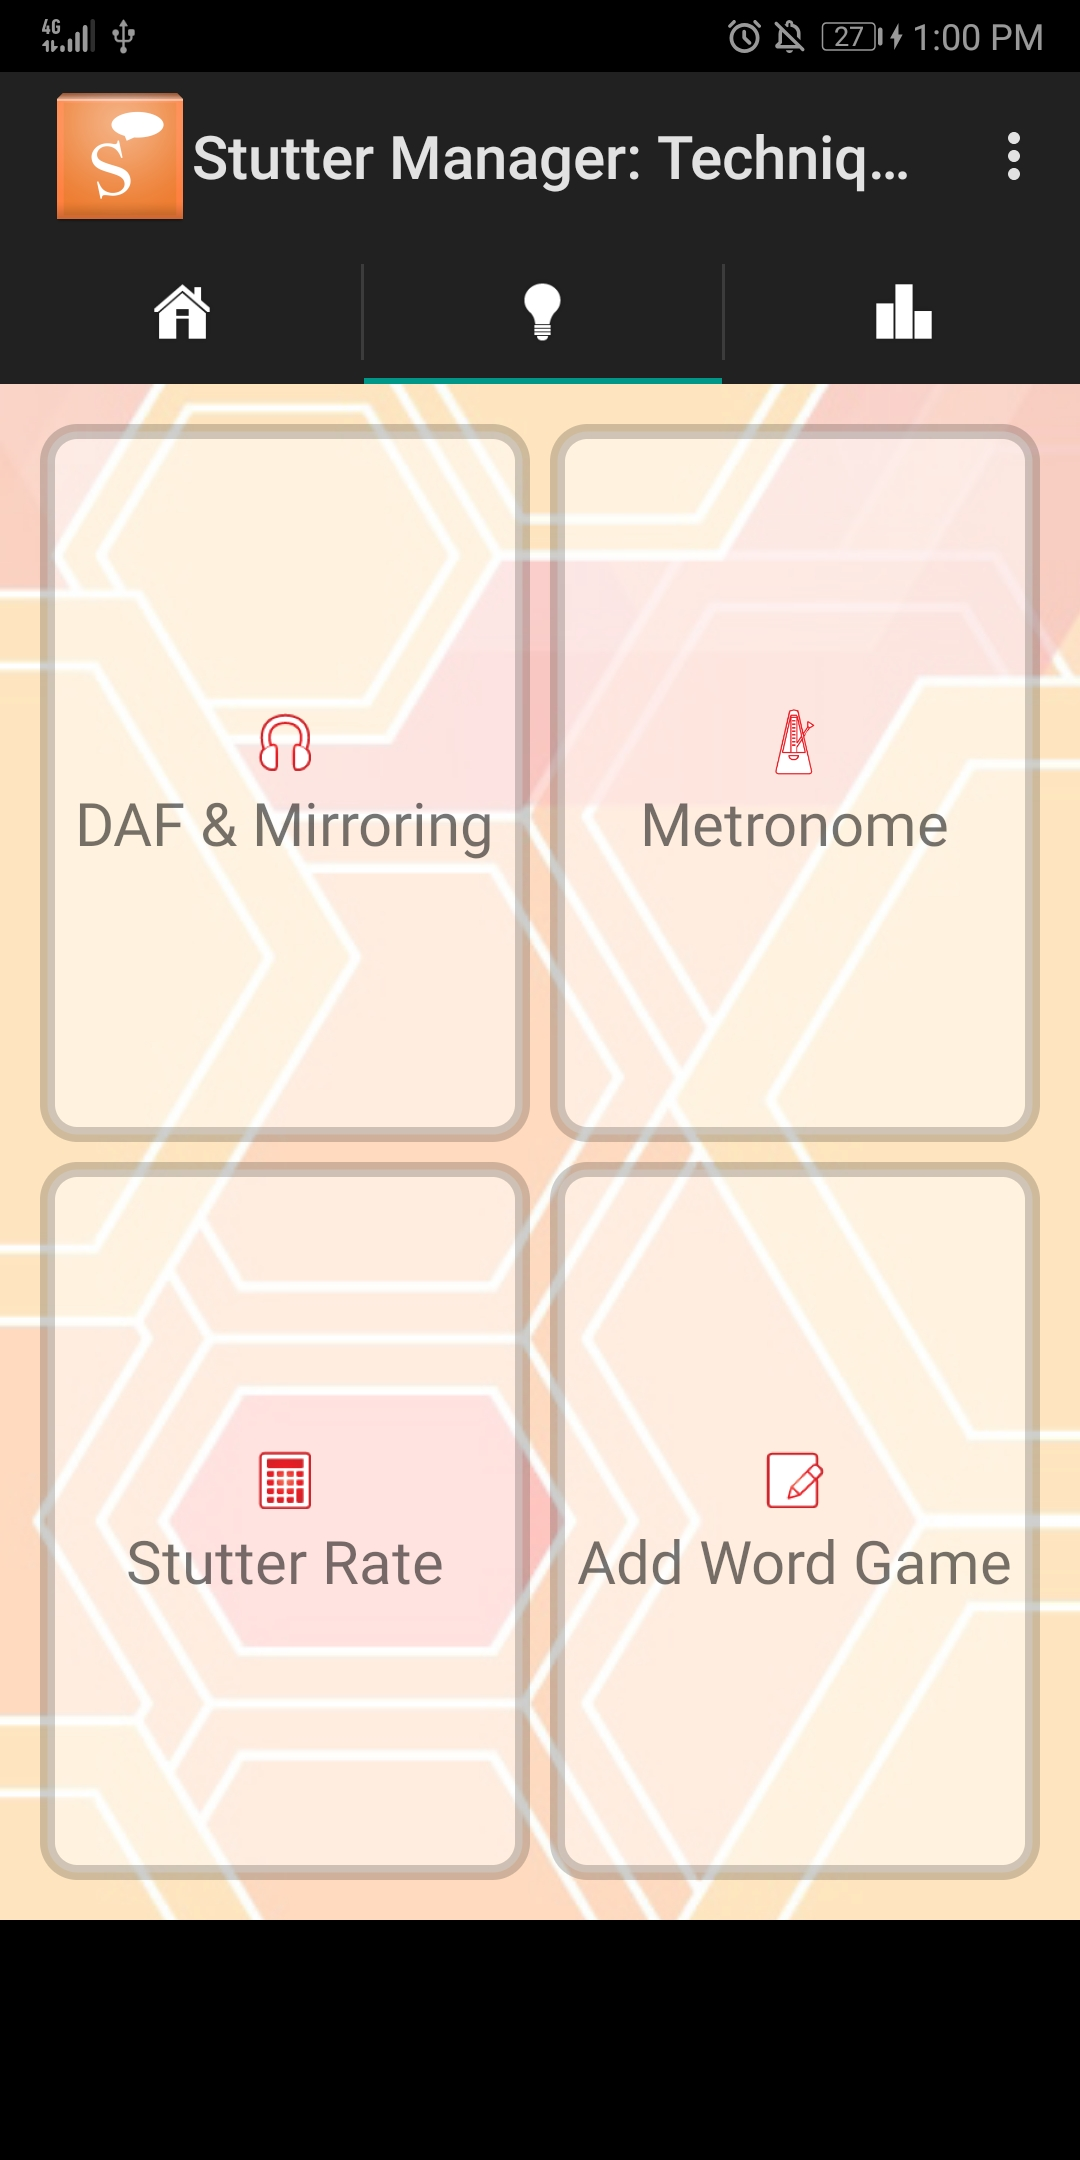
\includegraphics[width=.75\linewidth]{content/imgs/old_app_1.jpg}
    \caption{Page principale (exercices)}
  \end{subfigure}%
  \begin{subfigure}{.25\textwidth}
    \centering
    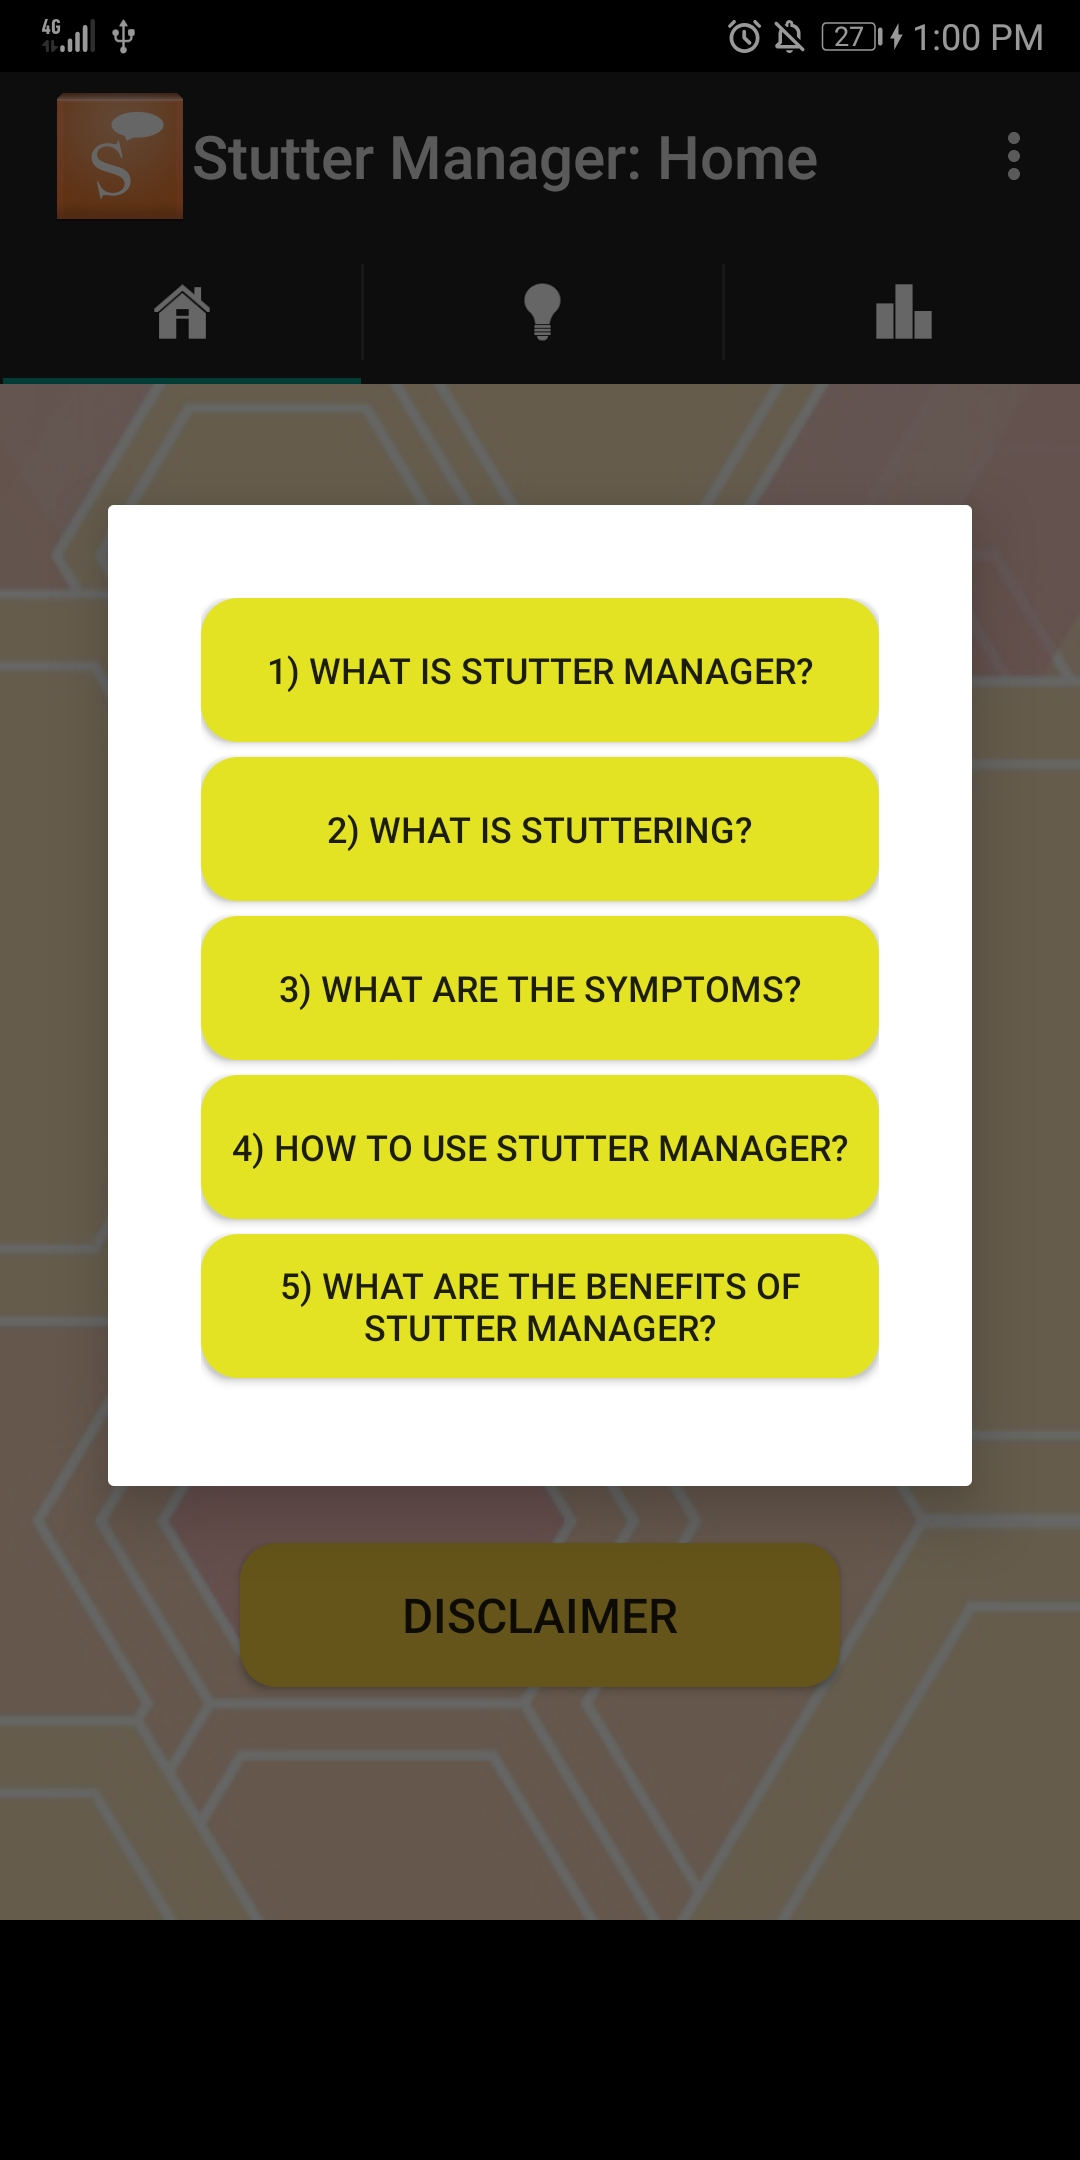
\includegraphics[width=.75\linewidth]{content/imgs/old_app_2.jpg}
    \caption{Informations générales}
  \end{subfigure}%
  \begin{subfigure}{.25\textwidth}
    \centering
    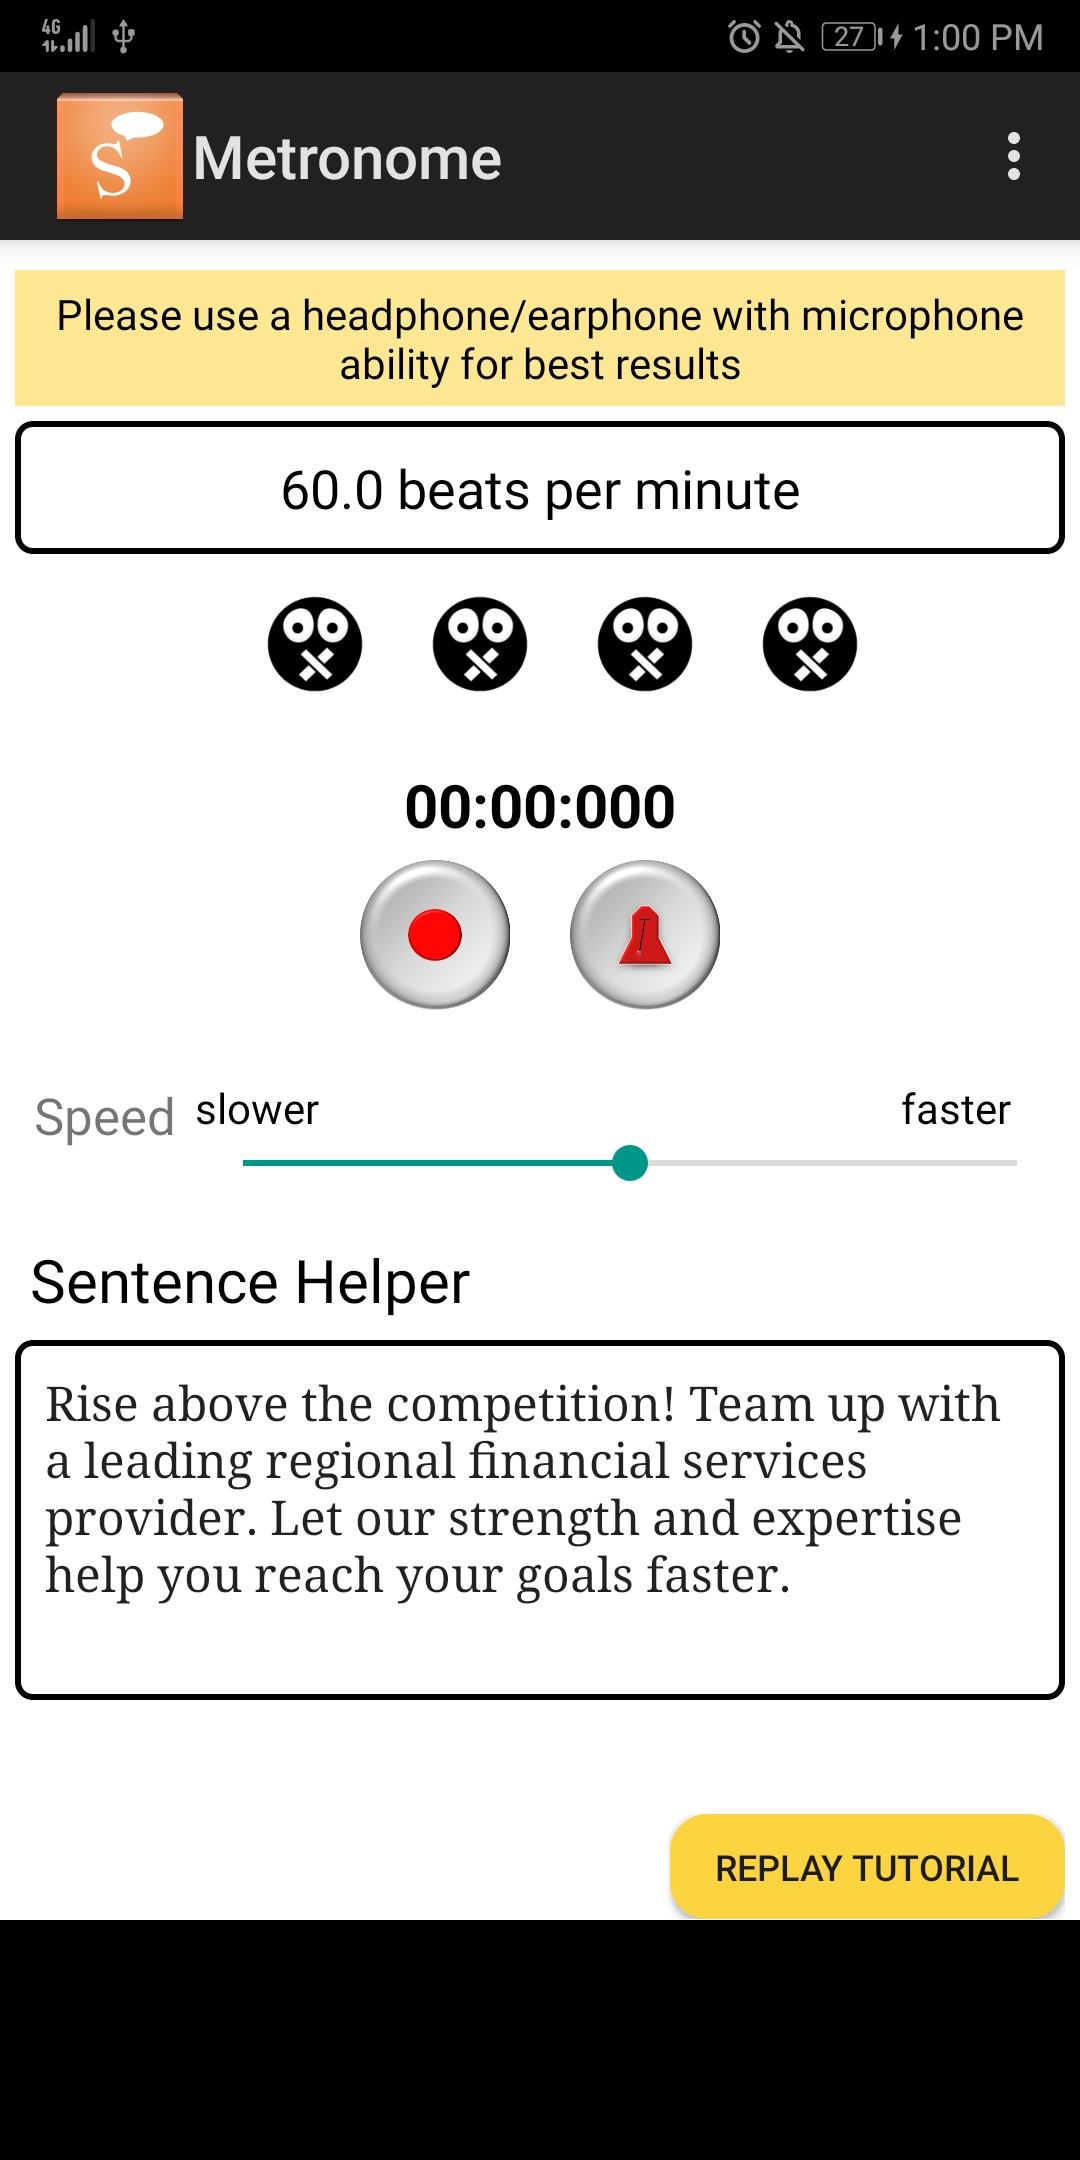
\includegraphics[width=.75\linewidth]{content/imgs/old_app_3.jpg}
    \caption{Exercice : Metronome}
  \end{subfigure}%
  \begin{subfigure}{.25\textwidth}
    \centering
    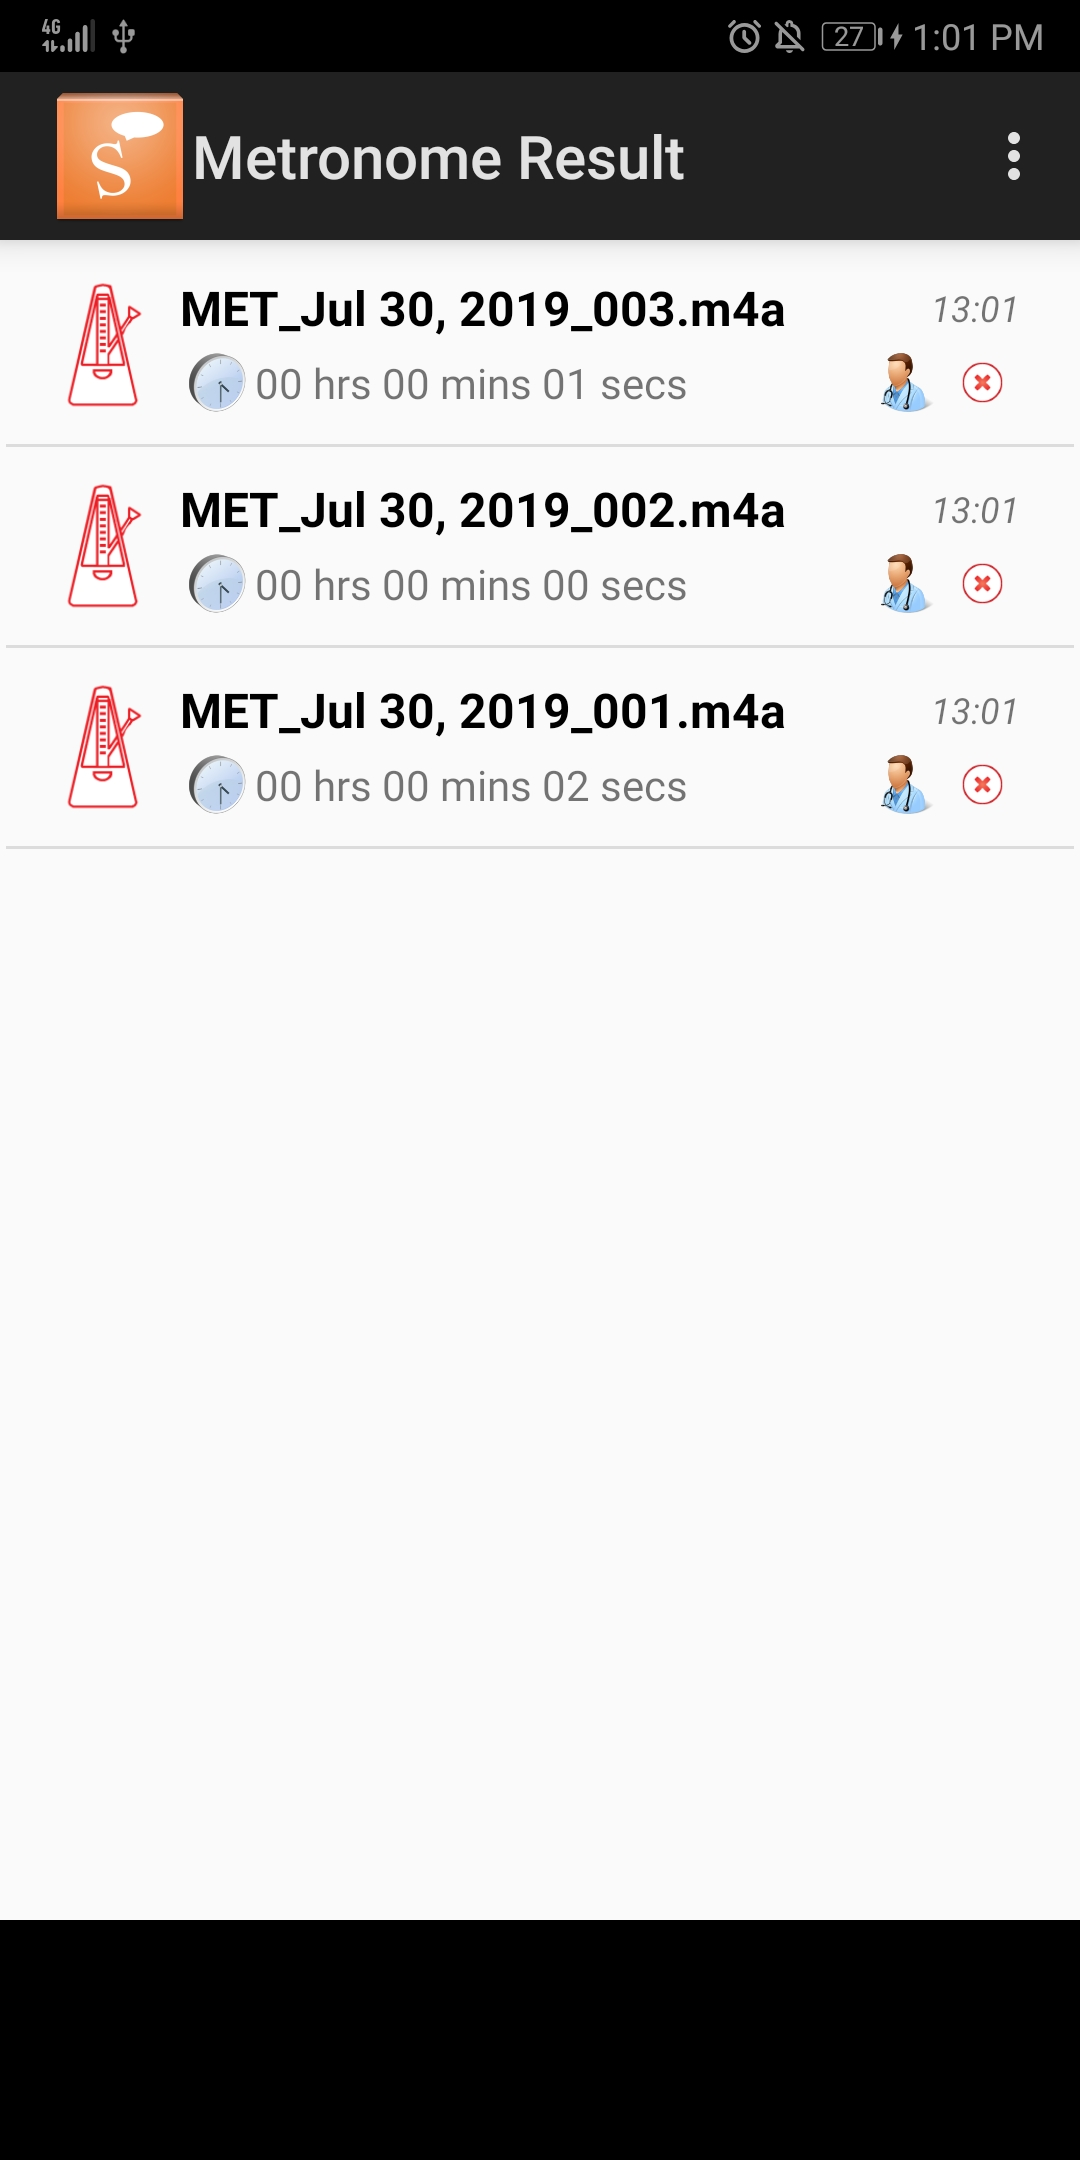
\includegraphics[width=.75\linewidth]{content/imgs/old_app_4.jpg}
    \caption{Progression de l'exercice metronome}
  \end{subfigure}
  \caption*{Captures d'écran de Stutter Manager v3}
\end{figure}

\end{landscape}




\chapter{Étude comparative}
\label{appendix:market}
\begin{figure}[h]
  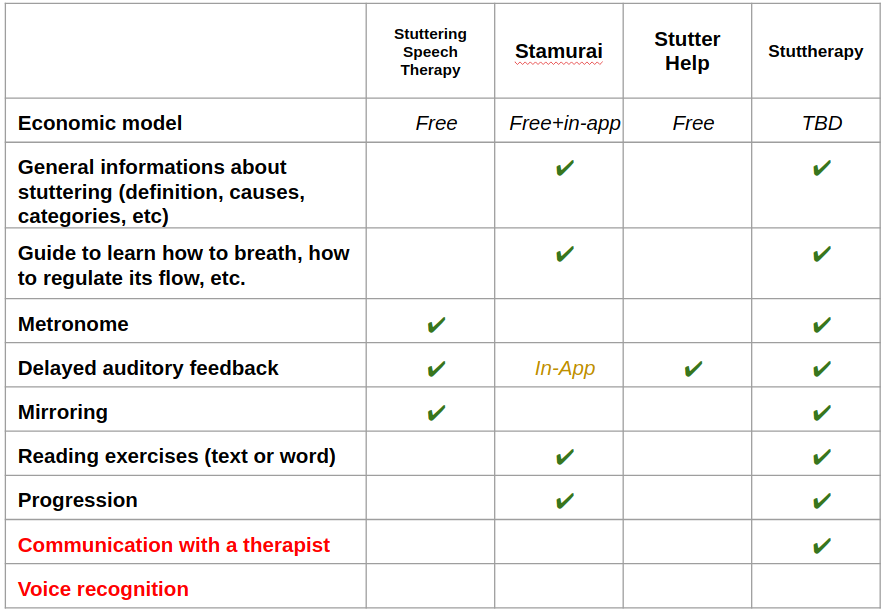
\includegraphics[width=1\linewidth]{content/imgs/market.png}
  \caption*{Étude comparative des applications disponibles sur le Play Store en comparaison avec les fonctionnalités prévues pour Stuttherapy}
\end{figure}



\chapter{Software requirements specification}
\label{appendix:srs}
\begin{figure}[h]
  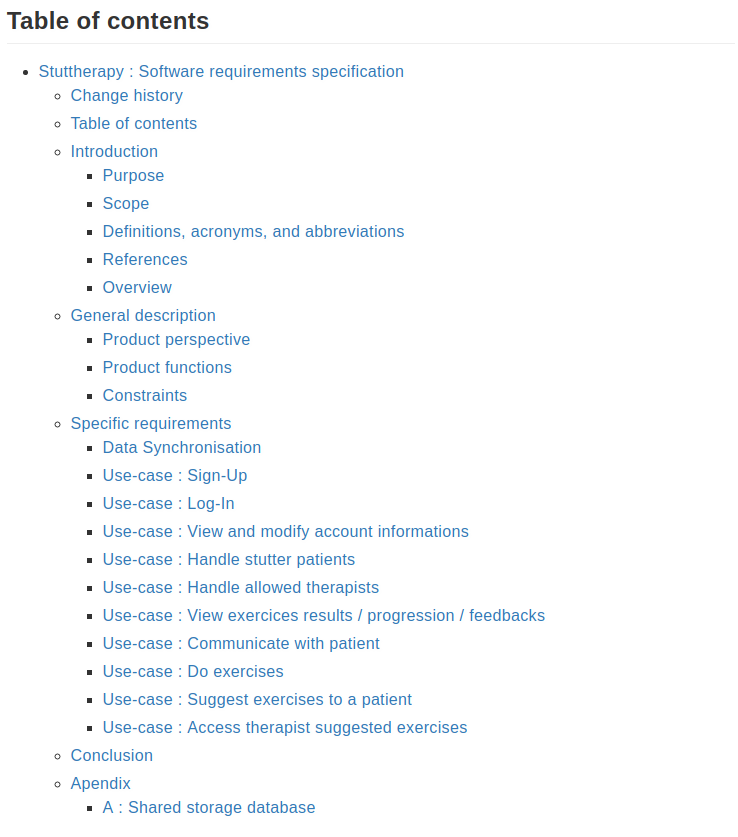
\includegraphics[width=0.7\linewidth]{content/imgs/srs_contents.png}
  \caption*{Table des matières du \textit{Software requirements specification}}
\end{figure}

\begin{displayquote}
The software requirements specification lays out functional and non-functional requirements, and it may include a set of use cases that describe user interactions that the software must provide to the user for perfect interaction.
\end{displayquote}
\hspace*{\fill} \textit{Wikipedia - Software Requirements Specification}


\begin{displayquote}
La spécification des exigences logicielles définit les exigences fonctionnelles et non fonctionnelles. Elle peut inclure un ensemble de cas d'utilisation décrivant les interactions de l'utilisateur que le logiciel doit fournir à l'utilisateur pour obtenir une interaction parfaite.
\end{displayquote}
\hspace*{\fill} \textit{Traduction du passage ci-dessus}


\chapter{Software requirements specifications - Exemple d'un cas d'utilisation}
\label{appendix:srs_example}
\begin{figure}[h]
  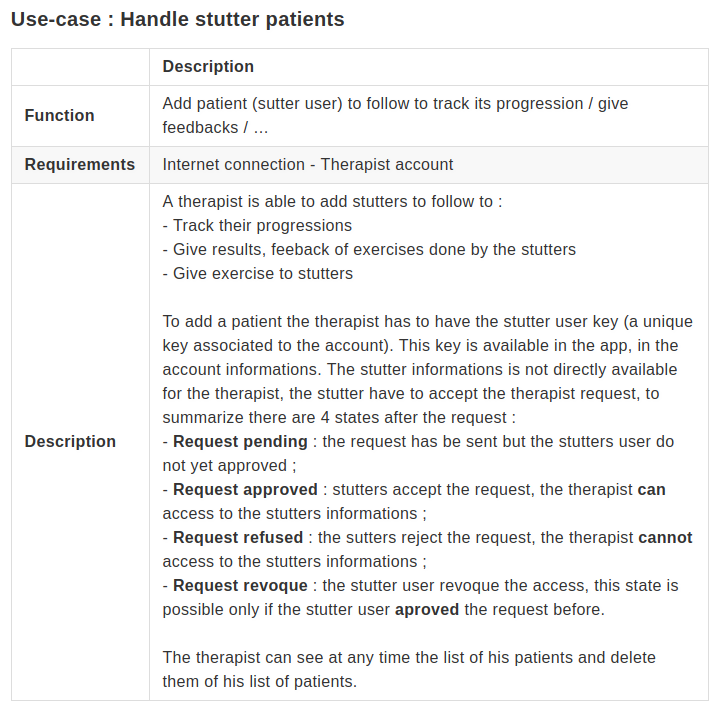
\includegraphics[width=1\linewidth]{content/imgs/srs_use_case_ex.png}
  \caption*{Spécification du cas d'utilisation \textbf{Handle stutter patients}}
\end{figure}




\begin{landscape}
  \label{appendix:gantt}
  \chapter{Diagramme de Gantt prévisionnel}
  \begin{figure}[H]
    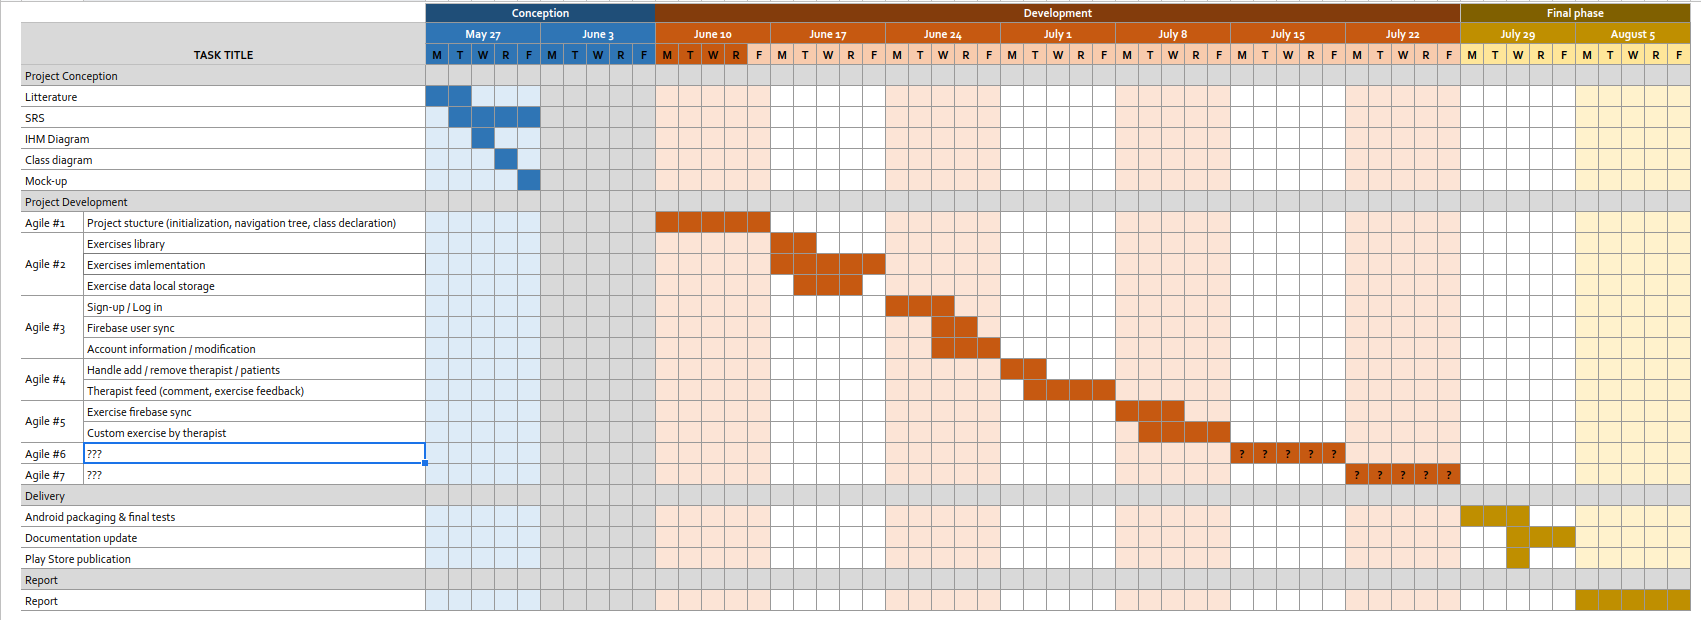
\includegraphics[width=1\linewidth]{content/imgs/gantt.png}
    \caption*{Diagramme de Gantt prévisionnel}
  \end{figure}
\end{landscape}


\chapter{Exemple release Github}
\label{appendix:release}
\begin{figure}[H]
  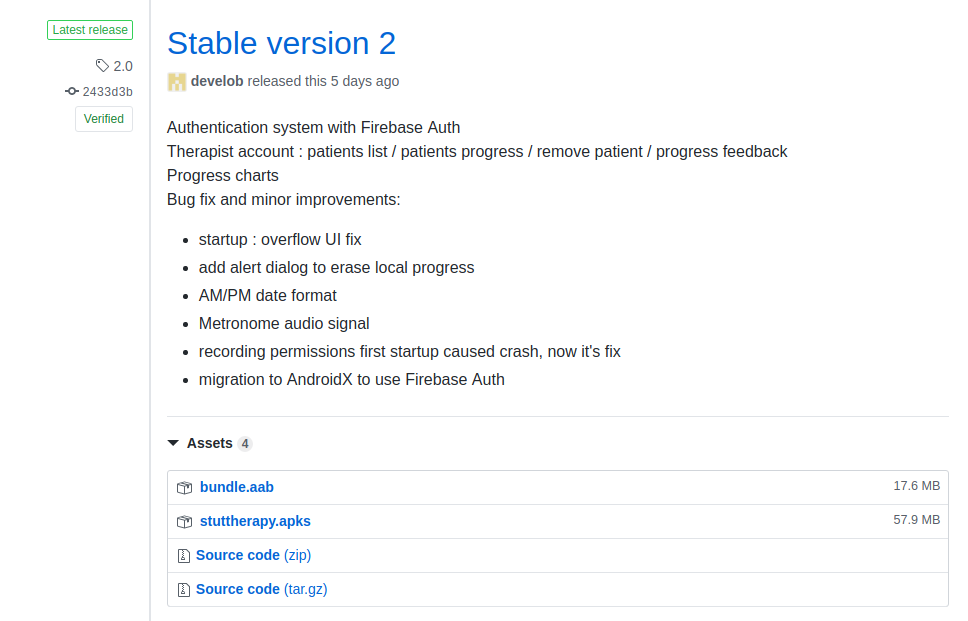
\includegraphics[width=1\linewidth]{content/imgs/release_ex.png}
  \caption*{Release finale de l'application}
\end{figure}

\chapter{Diagramme IHM}
\label{appendix:ihm}
\begin{figure}[H]
  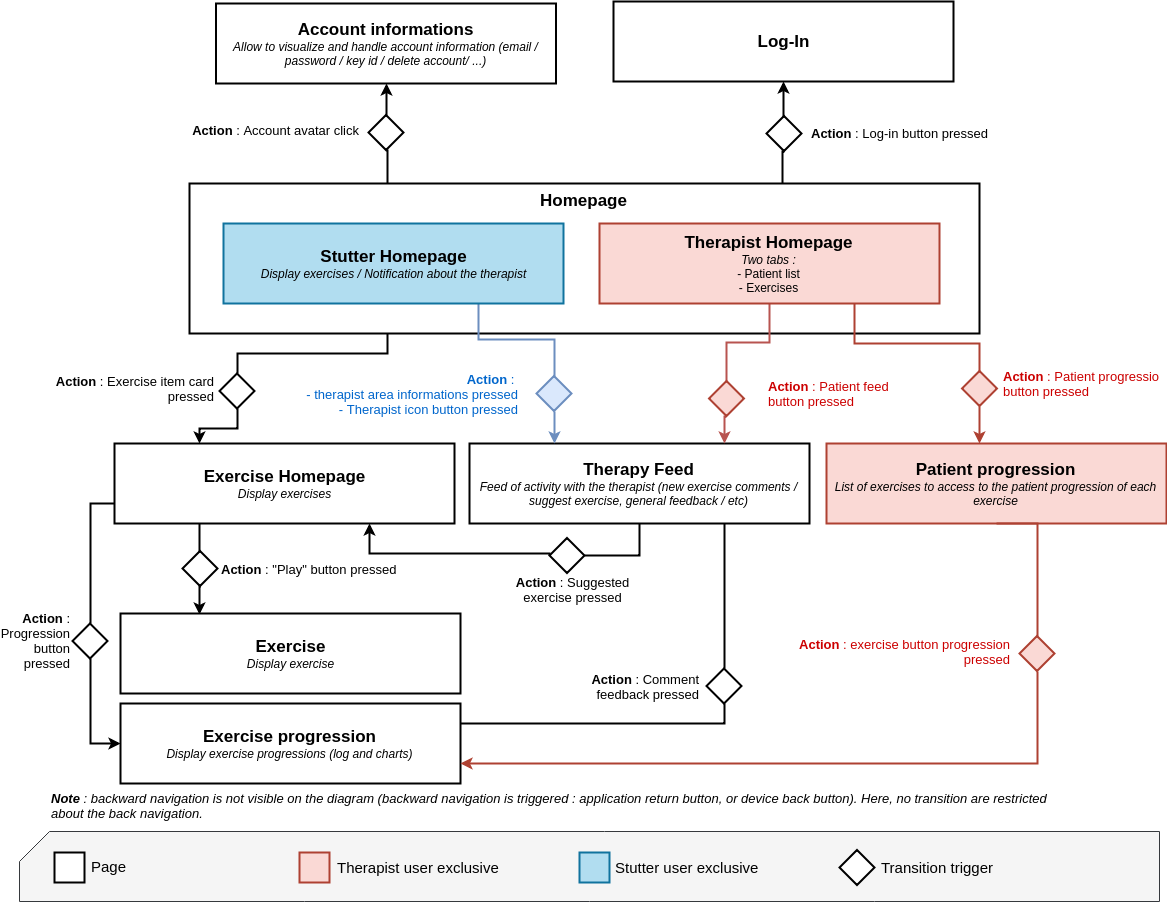
\includegraphics[width=1\linewidth]{content/imgs/IHM_diagram.png}
  \caption*{Diagramme IHM}
\end{figure}


\chapter{Wireframes}
\label{appendix:wireframes}
\section{Page principales}
\begin{figure}[H]
  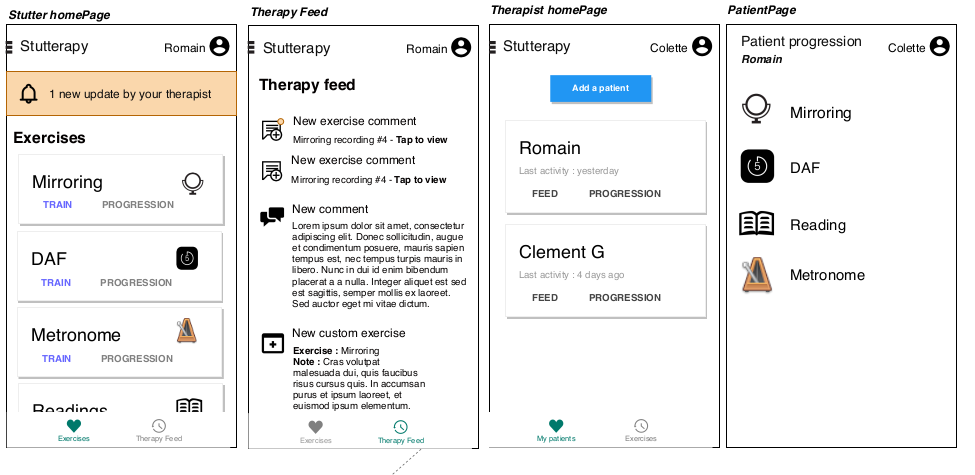
\includegraphics[width=1\linewidth]{content/imgs/maquette1.png}
  \caption*{Pages principales des bègues et des orthopédistes}
\end{figure}

\section{Exercices}
\begin{figure}[H]
  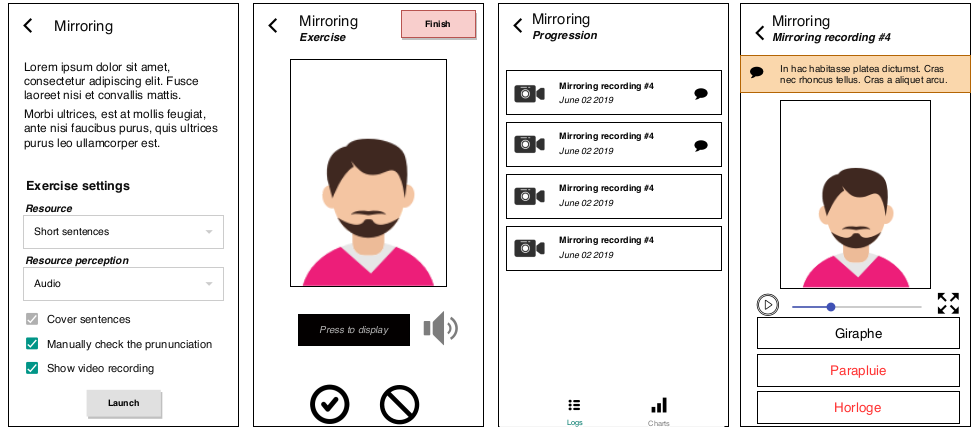
\includegraphics[width=1\linewidth]{content/imgs/maquette2a.png}
  \caption*{Exercice : Mirroring}
\end{figure}

\begin{figure}[H]
  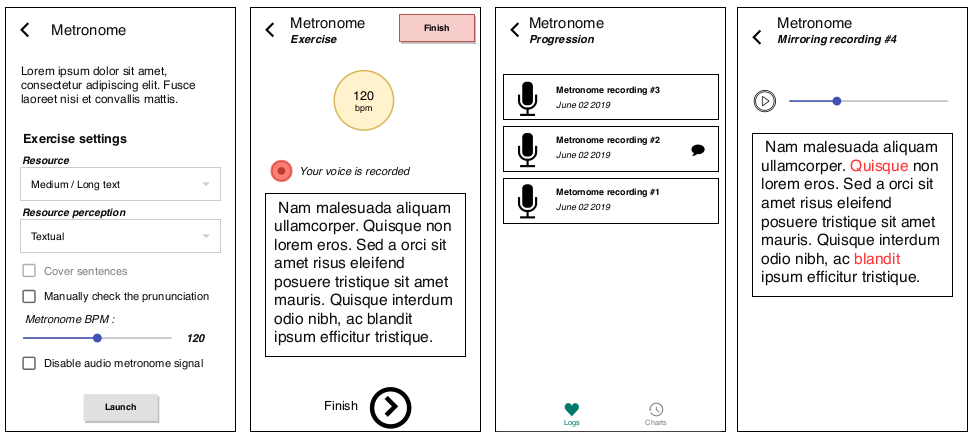
\includegraphics[width=1\linewidth]{content/imgs/maquette2b.png}
  \caption*{Exercice : Metronome}
\end{figure}

\begin{figure}[H]
  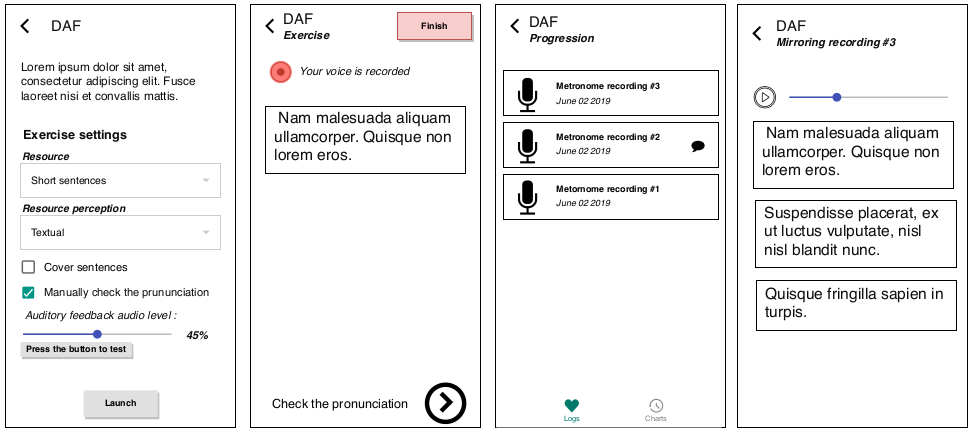
\includegraphics[width=1\linewidth]{content/imgs/maquette2c.png}
  \caption*{Exercice : DAF (delayed auditory feedback)}
\end{figure}

\begin{figure}[H]
  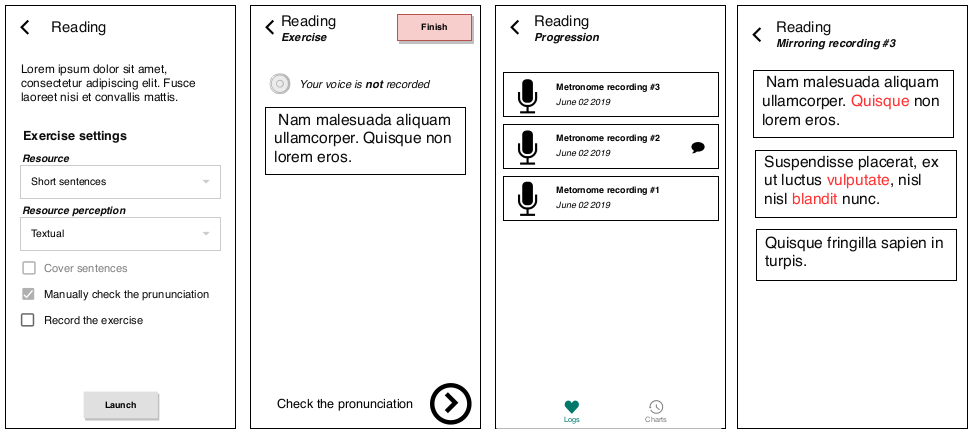
\includegraphics[width=1\linewidth]{content/imgs/maquette2d.png}
  \caption*{Exercice : Reading}
\end{figure}

\section{Divers}
\begin{figure}[H]
  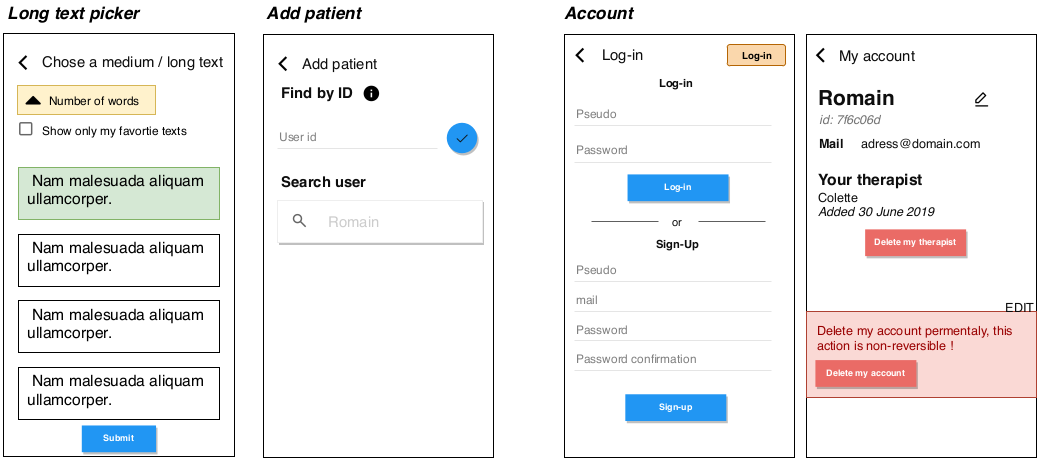
\includegraphics[width=1\linewidth]{content/imgs/maquette3.png}
  \caption*{Sélecteur de texte / ajout d'un patient / informations sur le compte}
\end{figure}






\begin{landscape}
\chapter{Diagramme de classe}
\label{appendix:class}
\vspace{-35pt}
\begin{figure}[H]
  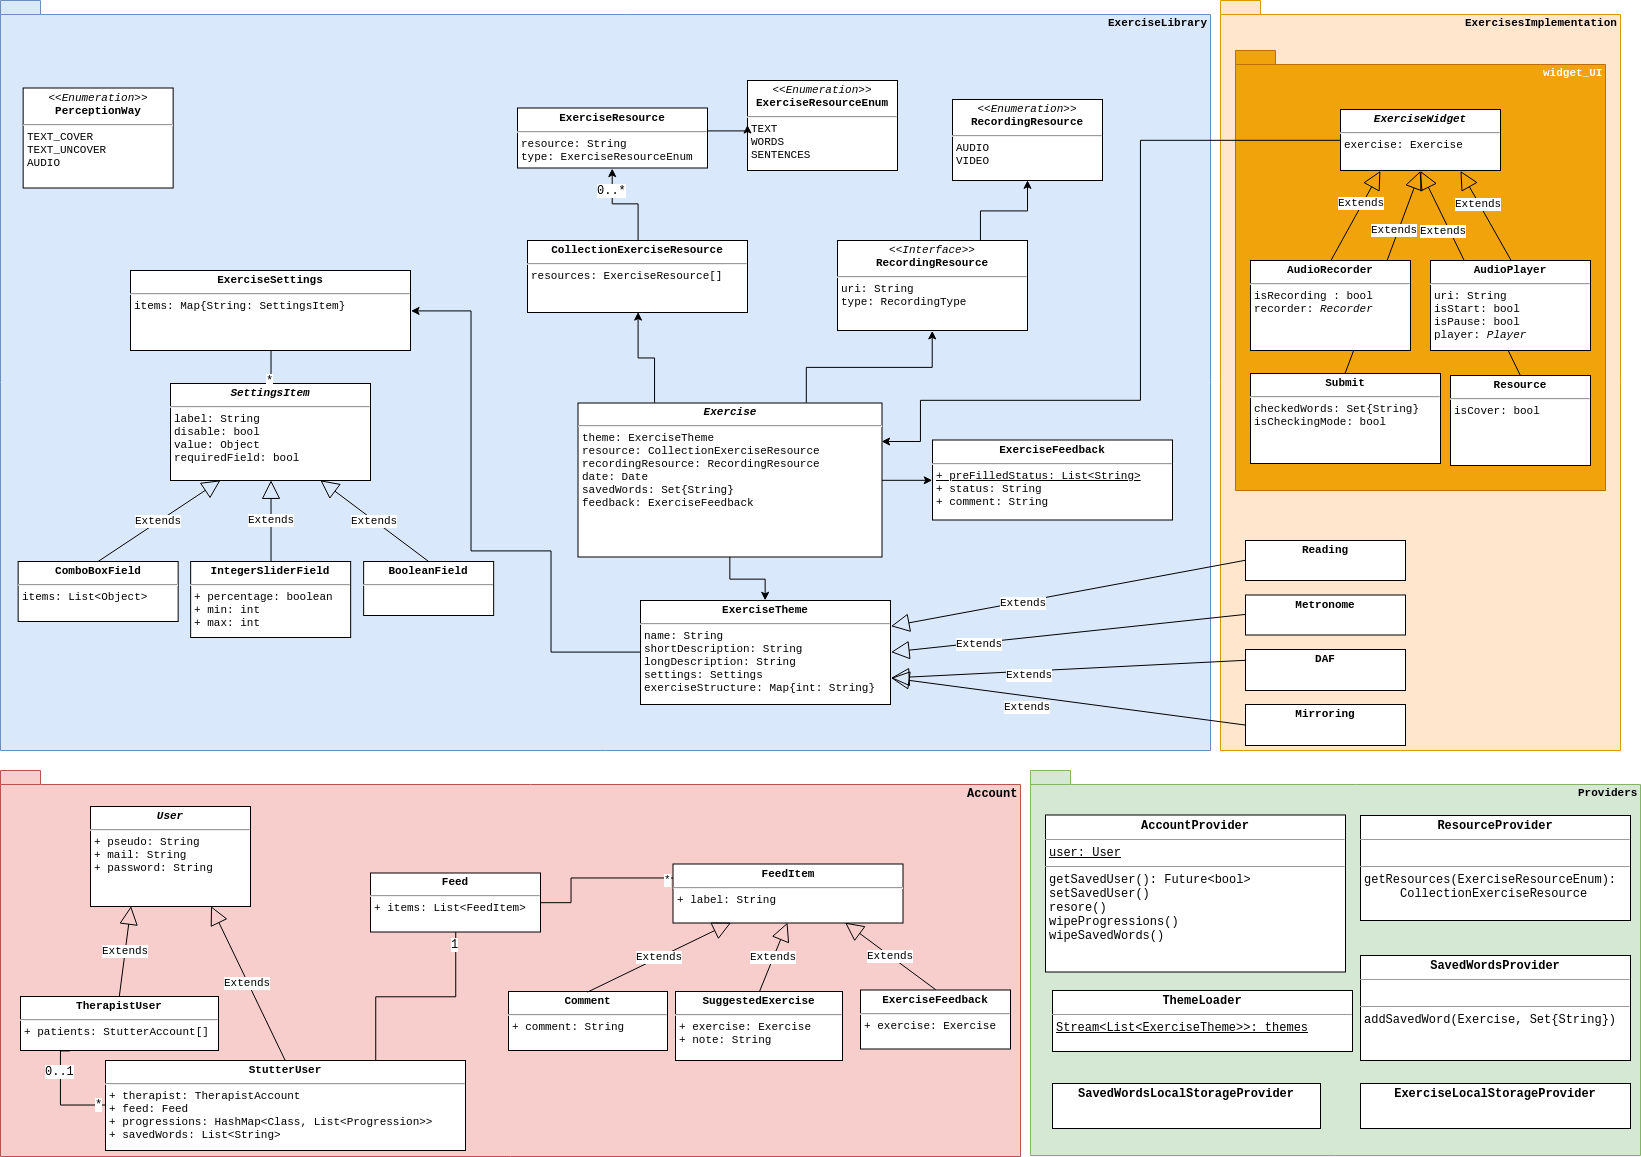
\includegraphics[width=0.9\linewidth]{content/imgs/app_class_diagram.png}
  \caption*{Diagramme IHM}
\end{figure}
\end{landscape}

\chapter{Stuttherapy - Captures d'écran}
\label{appendix:screenshots}




\end{appendices}
